~~~~Bayesian networks (BN) are graphical models where nodes represent random variables and arrows represent probabilistic dependencies
between them (Korb and Nicholson 2010).

A $n$-dimensional Bayesian network is a triple $B = (X, G, \Theta)$ where:

\begin{itemize}
	\item $X$ is a $n$-dimensional finite random vector each random variable $X_{i}$ ranges over by a finite domain $D_{i}$. Henceforward, we denote the joint domain by $D=\prod_{i=1}^{n}D_{i}$
	
	\item $G = (N, E)$ is a directed acyclic graph (DAG) with nodes $N = \{X_{1}, \cdots, X_{n}\}$ and edges $E$ representing direct dependencies between the variables.
	
	\item $\Theta$ encodes the parameters $\{\theta_{ijk}\}_{i\in1,\cdots,n,j\in D_{\prod_{X_{i}}},k\in D_{i}}$ of the network, where
	$$\theta_{ijk}=P_{B}(X_{i}=x_{ik}|\prod_{X_{i}}=\omega_{ij}),$$
	
	$\prod_{X_{i}}$ denotes the set of parents of $X_{i}$ in $G$, $D_{\prod_{X_{i}}}$ denotes the joint domain of the variables in $\prod_{X_{i}, x_{ik}}$ is the $k$-th value of $X_{i}$ and $\omega_{ij}$ is the $j$-th configuration of $\prod_{X_{i}}$.
\end{itemize}

\begin{figure}[!h]
	\centering
		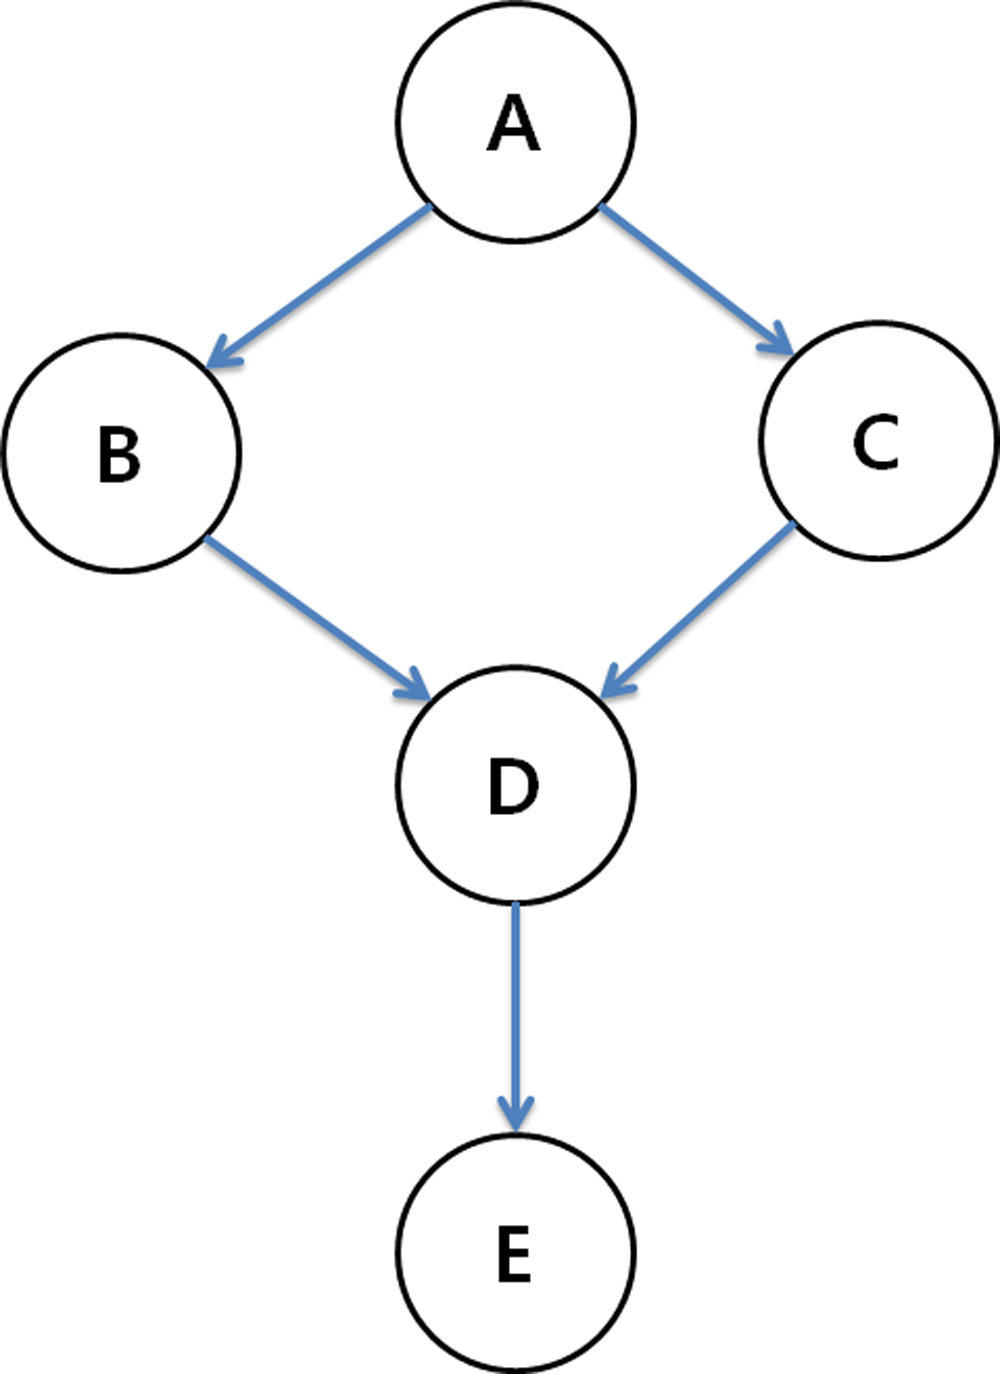
\includegraphics[height=150pt]{image01}
		\caption{$P(A,B,C,D,E)=P(A)P(B|A)P(C|A)P(D|B,C)P(E|D)$}
\end{figure}	

A BN defines a unique joint probability distribution over $X$ given by
$$P_{B}(X_{1},\cdots,X_{n})=\prod_{i=1}^{n}P_{B}(X_{i}|\prod_{X_{i}}).$$

\begin{itemize}
	\item A BN encodes the independence assumptions over the component random variables of $X$.
	
	\item An edge $(j, i)$ in $E$ represents a direct dependency of $X_{i}$ from $X_{j}$.
	
	\item The set of all Bayesian networks with $n$ variables is denotes by $B_{n}$.
\end{itemize}
